% Options for packages loaded elsewhere
\PassOptionsToPackage{unicode}{hyperref}
\PassOptionsToPackage{hyphens}{url}
\PassOptionsToPackage{dvipsnames,svgnames*,x11names*}{xcolor}
%
\documentclass[
  12pt,
  a4paper,
  xelatex,
  ja=standard]{bxjsarticle}
\usepackage{amsmath,amssymb}
\usepackage{lmodern}
\usepackage{setspace}
\usepackage{ifxetex,ifluatex}
\ifnum 0\ifxetex 1\fi\ifluatex 1\fi=0 % if pdftex
  \usepackage[T1]{fontenc}
  \usepackage[utf8]{inputenc}
  \usepackage{textcomp} % provide euro and other symbols
\else % if luatex or xetex
  \usepackage{unicode-math}
  \defaultfontfeatures{Scale=MatchLowercase}
  \defaultfontfeatures[\rmfamily]{Ligatures=TeX,Scale=1}
\fi
% Use upquote if available, for straight quotes in verbatim environments
\IfFileExists{upquote.sty}{\usepackage{upquote}}{}
\IfFileExists{microtype.sty}{% use microtype if available
  \usepackage[]{microtype}
  \UseMicrotypeSet[protrusion]{basicmath} % disable protrusion for tt fonts
}{}
\makeatletter
\@ifundefined{KOMAClassName}{% if non-KOMA class
  \IfFileExists{parskip.sty}{%
    \usepackage{parskip}
  }{% else
    \setlength{\parindent}{0pt}
    \setlength{\parskip}{6pt plus 2pt minus 1pt}}
}{% if KOMA class
  \KOMAoptions{parskip=half}}
\makeatother
\usepackage{xcolor}
\IfFileExists{xurl.sty}{\usepackage{xurl}}{} % add URL line breaks if available
\IfFileExists{bookmark.sty}{\usepackage{bookmark}}{\usepackage{hyperref}}
\hypersetup{
  pdftitle={PDF Document Template, BXjs Class},
  pdfauthor={Your Name, Licence},
  colorlinks=true,
  linkcolor=Maroon,
  filecolor=Maroon,
  citecolor=Blue,
  urlcolor=Blue,
  pdfcreator={LaTeX via pandoc}}
\urlstyle{same} % disable monospaced font for URLs
\usepackage{color}
\usepackage{fancyvrb}
\newcommand{\VerbBar}{|}
\newcommand{\VERB}{\Verb[commandchars=\\\{\}]}
\DefineVerbatimEnvironment{Highlighting}{Verbatim}{commandchars=\\\{\}}
% Add ',fontsize=\small' for more characters per line
\usepackage{framed}
\definecolor{shadecolor}{RGB}{248,248,248}
\newenvironment{Shaded}{\begin{snugshade}}{\end{snugshade}}
\newcommand{\AlertTok}[1]{\textcolor[rgb]{0.94,0.16,0.16}{#1}}
\newcommand{\AnnotationTok}[1]{\textcolor[rgb]{0.56,0.35,0.01}{\textbf{\textit{#1}}}}
\newcommand{\AttributeTok}[1]{\textcolor[rgb]{0.77,0.63,0.00}{#1}}
\newcommand{\BaseNTok}[1]{\textcolor[rgb]{0.00,0.00,0.81}{#1}}
\newcommand{\BuiltInTok}[1]{#1}
\newcommand{\CharTok}[1]{\textcolor[rgb]{0.31,0.60,0.02}{#1}}
\newcommand{\CommentTok}[1]{\textcolor[rgb]{0.56,0.35,0.01}{\textit{#1}}}
\newcommand{\CommentVarTok}[1]{\textcolor[rgb]{0.56,0.35,0.01}{\textbf{\textit{#1}}}}
\newcommand{\ConstantTok}[1]{\textcolor[rgb]{0.00,0.00,0.00}{#1}}
\newcommand{\ControlFlowTok}[1]{\textcolor[rgb]{0.13,0.29,0.53}{\textbf{#1}}}
\newcommand{\DataTypeTok}[1]{\textcolor[rgb]{0.13,0.29,0.53}{#1}}
\newcommand{\DecValTok}[1]{\textcolor[rgb]{0.00,0.00,0.81}{#1}}
\newcommand{\DocumentationTok}[1]{\textcolor[rgb]{0.56,0.35,0.01}{\textbf{\textit{#1}}}}
\newcommand{\ErrorTok}[1]{\textcolor[rgb]{0.64,0.00,0.00}{\textbf{#1}}}
\newcommand{\ExtensionTok}[1]{#1}
\newcommand{\FloatTok}[1]{\textcolor[rgb]{0.00,0.00,0.81}{#1}}
\newcommand{\FunctionTok}[1]{\textcolor[rgb]{0.00,0.00,0.00}{#1}}
\newcommand{\ImportTok}[1]{#1}
\newcommand{\InformationTok}[1]{\textcolor[rgb]{0.56,0.35,0.01}{\textbf{\textit{#1}}}}
\newcommand{\KeywordTok}[1]{\textcolor[rgb]{0.13,0.29,0.53}{\textbf{#1}}}
\newcommand{\NormalTok}[1]{#1}
\newcommand{\OperatorTok}[1]{\textcolor[rgb]{0.81,0.36,0.00}{\textbf{#1}}}
\newcommand{\OtherTok}[1]{\textcolor[rgb]{0.56,0.35,0.01}{#1}}
\newcommand{\PreprocessorTok}[1]{\textcolor[rgb]{0.56,0.35,0.01}{\textit{#1}}}
\newcommand{\RegionMarkerTok}[1]{#1}
\newcommand{\SpecialCharTok}[1]{\textcolor[rgb]{0.00,0.00,0.00}{#1}}
\newcommand{\SpecialStringTok}[1]{\textcolor[rgb]{0.31,0.60,0.02}{#1}}
\newcommand{\StringTok}[1]{\textcolor[rgb]{0.31,0.60,0.02}{#1}}
\newcommand{\VariableTok}[1]{\textcolor[rgb]{0.00,0.00,0.00}{#1}}
\newcommand{\VerbatimStringTok}[1]{\textcolor[rgb]{0.31,0.60,0.02}{#1}}
\newcommand{\WarningTok}[1]{\textcolor[rgb]{0.56,0.35,0.01}{\textbf{\textit{#1}}}}
\usepackage{graphicx}
\makeatletter
\def\maxwidth{\ifdim\Gin@nat@width>\linewidth\linewidth\else\Gin@nat@width\fi}
\def\maxheight{\ifdim\Gin@nat@height>\textheight\textheight\else\Gin@nat@height\fi}
\makeatother
% Scale images if necessary, so that they will not overflow the page
% margins by default, and it is still possible to overwrite the defaults
% using explicit options in \includegraphics[width, height, ...]{}
\setkeys{Gin}{width=\maxwidth,height=\maxheight,keepaspectratio}
% Set default figure placement to htbp
\makeatletter
\def\fps@figure{htbp}
\makeatother
% Make links footnotes instead of hotlinks:
\DeclareRobustCommand{\href}[2]{#2\footnote{\url{#1}}}
\setlength{\emergencystretch}{3em} % prevent overfull lines
\providecommand{\tightlist}{%
  \setlength{\itemsep}{0pt}\setlength{\parskip}{0pt}}
\setcounter{secnumdepth}{5}
% --- BXjsクラス用 ------------------------------------------------------------
% https://ctan.math.washington.edu/tex-archive/language/japanese/BX/bxjscls/bxjscls-manual.pdf
% --- 参考資料 ----------------------------------------------------------------
% https://github.com/Gedevan-Aleksizde/Japan.R2019/blob/master/latex/preamble.tex
% https://teastat.blogspot.com/2019/01/bookdown.html

% --- Document Class ----------------------------------------------------------
% Rmd側で指定した方が分かりやすいかも
% \documentclass[a4paper,xelatex,ja=standard]{bxjsarticle}

% --- Packages ----------------------------------------------------------------
% 日本語とkableExtraを使うために必要なTeXパッケージ指定
%  A4 210mm x 297mm
% \usepackage[a4paper]{geometry}         % Rmdのclassoptionでも指定可能
\usepackage{indentfirst}               % tinytexのリポジトリには存在しない?
\usepackage{booktabs}                  % ここからkableExtra用パッケージ
\usepackage{longtable}                 % 1 column modeのみで利用可
\usepackage{array}                     % 
\usepackage{multirow}                  % 
\usepackage{wrapfig}                   % 
\usepackage{float}                     % 
\usepackage{colortbl}                  % 
\usepackage{pdflscape}                 % 
\usepackage{tabu}                      % 
\usepackage{threeparttable}            % 
\usepackage{threeparttablex}           % 
\usepackage[normalem]{ulem}            % 
\usepackage{inputenc}                  % 
\usepackage{makecell}                  % 
\usepackage{xcolor}                    % ここまでkableExtra用
\usepackage{amsmath}                   % 
\usepackage{fontawesome5}              % fontawesomeを使うために必要
\usepackage{subfig}                    % 複数の図を並べる際に必要(古い?)
% \usepackage{subcaption}                % 同上(新しい?)
\usepackage{zxjatype}                  % 日本語処理に必要
% \usepackage{xeCJK}                     % zxjatypeを読み込むと自動で読み込む
\usepackage[noto]{zxjafont}            % Linux環境ではこちも使える
% \usepackage[haranoaji]{zxjafont}       % Windows環境ではこちらだけ
% \usepackage[hiragino-pro]{zxjafont}    % macOS環境用(おそらく、駄目ならNotoで)
\usepackage{pxrubrica}                 % ルビ用
\usepackage{hyperref}                  % ハイパーリンク用必要?


% --- Page layout -------------------------------------------------------------
% http://joker.hatenablog.com/entry/2012/07/09/153537
% \usepackage{layout}

% \setpagelayout*{margin=25truemm}
% \setpagelayout*{top=20truemm,bottom=20truemm,left=25truemm,right=25truemm}

% --- Page Header -------------------------------------------------------------
% \usepackage{fancyhdr}
% \pagestyle{fancy}
% \lhead{}
% \rhead{\bf\thepage}

% --- Bookdownによる技術系同人誌執筆 ------------------------------------------
% https://teastat.blogspot.com/2019/01/bookdown.html
% \makeatletter
% \def\emptypage@emptypage{%
%     \hbox{}%
%     \thispagestyle{headings}%
%     \newpage%    
% }%
% \def\cleardoublepage{%
%         \clearpage%
%         \if@twoside%
%             \ifodd\c@page%
%                 % do nothing
%             \else%
%                 \emptypage@emptypage%
%             \fi%
%         \fi%
%     }%
% \makeatother
\usepackage{booktabs}
\usepackage{longtable}
\usepackage{array}
\usepackage{multirow}
\usepackage{wrapfig}
\usepackage{float}
\usepackage{colortbl}
\usepackage{pdflscape}
\usepackage{tabu}
\usepackage{threeparttable}
\usepackage{threeparttablex}
\usepackage[normalem]{ulem}
\usepackage{makecell}
\usepackage{xcolor}
\ifluatex
  \usepackage{selnolig}  % disable illegal ligatures
\fi

\title{PDF Document Template, BXjs Class}
\author{Your Name, Licence}
\date{2021-06-03}

\begin{document}
\maketitle
\begin{abstract}
本ファイルはデフォルトのPDFテンプレートにおいて日本語が使えるような設定を施してあります。必ず同梱の\texttt{latex}フォルダと同じ階層に配置してください。
\end{abstract}

\setstretch{0.85}
\hypertarget{ux672cux30c6ux30f3ux30d7ux30ecux30fcux30c8ux306eux4f7fux3044ux65b9}{%
\section{本テンプレートの使い方}\label{ux672cux30c6ux30f3ux30d7ux30ecux30fcux30c8ux306eux4f7fux3044ux65b9}}

前提条件

\begin{itemize}
\tightlist
\item
  \textbf{\texttt{tidyverse}, \texttt{knitr}, \texttt{rmarkdown},
  \texttt{psych}, \texttt{kableExtra}}パッケージ\footnote{\textbf{R}
    4.x推奨}
\item
  \textbf{RStudio}\footnote{v1.4推奨}
\item
  \textbf{Notoフォント}(Linux)・\textbf{ヒラギノフォント}\footnote{検証していないので推測です}(macOS)
\end{itemize}

作成手順

\begin{enumerate}
\def\labelenumi{\arabic{enumi}.}
\tightlist
\item
  \textbf{\texttt{tinytex}}パッケージをインストールする
\item
  \texttt{tinytex::install\_tinytex()}で\textbf{tinytex}をインストールする
\item
  \texttt{tinytex::tlmgr\_install("haranoaji")}で原の味フォントをインストールする\footnote{Windows環境のみ}
\item
  \texttt{latex/tufte\_preamble.tex}を開いてOS環境に見合ったフォント設定を有効にする\footnote{不要な設定は\%文字でコメントアウトします}
\item
  本ドキュメントをknitする

  \begin{itemize}
  \tightlist
  \item
    必要なTeXパッケージは\textbf{tinytex}が自動的にインストールする
  \item
    もしTeXのメッセージが出た場合にはログを参考に必要なパッケージをインストール\footnote{\texttt{tinytex::tlmgr\_install("package")}を\textbf{RStudio}のコンソールから実行します}する
  \item
    出力フォーマットを変更したい場合はYAMLの\texttt{documentclass}指定を変更する
  \end{itemize}
\end{enumerate}

\hypertarget{ux5236ux9650ux4e8bux9805ux306aux3069}{%
\subsection{制限事項など}\label{ux5236ux9650ux4e8bux9805ux306aux3069}}

R
MarkdownでPDFを作成するのは簡単ですが、日本語を含んだPDFを作成するには様々な知識が必要です。特にTeXの知識がないと日本語の表示すらままなりません。特にWindows環境は経験的に厄介ですので基本的にサポートはありません。

\begin{itemize}
\item
  \textbf{tinytex}以外のTeX/LaTeXを利用する場合は手動でパッケージをインストールしてください

  \begin{itemize}
  \tightlist
  \item
    \textbf{tinytex}以外のTeX/LaTeXでの動作は確認していません
  \item
    \textbf{RStudio}でのLaTeXエンジン指定は必ず\texttt{xelatex}を指定してください
  \end{itemize}
\item
  本テンプレートは必要最低限の設定だけです

  \begin{itemize}
  \tightlist
  \item
    TeX/LaTeX\$のデフォルト仕様として図表は自動的に再配置されます
  \item
    図を位置固定したい場合は\texttt{setup}チャンク内の\texttt{fig.pos}オプションを試してください
  \item
    表を位置固定したい場合は定義してある\texttt{df\_print()}関数を試してください
  \item
    各種の指定方法は本ドキュメントに記述されています\footnote{\href{https://ftp.jaist.ac.jp/pub/CTAN/macros/latex/contrib/tufte-latex/sample-handout.pdf}{ドキュメントサンプル(PDF)}も参照してください}
  \end{itemize}
\item
  Winodws環境はレンダリングに時間がかかる場合があります
\item
  レンダリング時に\texttt{xeCJK}パッケージのワーニングが出ます\footnote{フォント設定を再設定しているだけなので特に問題はないかと\ldots{}}
\item
  平仮名の「う(U)」が表示されない問題があります\footnote{Linux環境で原ノ味フォントを指定した場合、Linux環境ではNotoフォントを指定してください}
\item
  レイアウト調整をしたい場合は\href{https://ctan.math.washington.edu/tex-archive/language/japanese/BX/bxjscls/bxjscls-manual.pdf}{BXjsclsユーザーマニュアル(PDF)}を参照してください
\item
  TeXの特殊文字(「\textbackslash TeX」など)は使えません\footnote{もしかしたらなにか指定方法があるのかも\ldots{}}

  \begin{itemize}
  \tightlist
  \item
    LaTeX数式モードは使えます
  \end{itemize}
\end{itemize}

enjoy!

\newpage

\hypertarget{ux72ecux81eaux306eux95a2ux6570ux5b9aux7fa9}{%
\section{独自の関数定義}\label{ux72ecux81eaux306eux95a2ux6570ux5b9aux7fa9}}

PDFではインタラクティブな表が使えません。また、tufteは余白が広いので通常の表出力では表示できる項目数が限られてしまいます。そこで、表現の自由度を高めるために\textbf{\texttt{kableExtra}}パッケージと\textbf{\texttt{psych}}パッケージを用いた\texttt{df\_print()}関数\footnote{詳細は\texttt{setup}チャンク内の関数が定義を参照方}を定義してあります。以下は使い方の一例です。

\begin{Shaded}
\begin{Highlighting}[numbers=left,,]
\NormalTok{mtcars[}\DecValTok{1}\SpecialCharTok{:}\DecValTok{6}\NormalTok{, }\DecValTok{1}\SpecialCharTok{:}\DecValTok{6}\NormalTok{] }\SpecialCharTok{\%\textgreater{}\%} 
  \FunctionTok{df\_print}\NormalTok{(}\AttributeTok{caption =} \StringTok{"デフォルトの表示方法です"}\NormalTok{)}
\end{Highlighting}
\end{Shaded}

\begin{table}[H]

\caption{\label{tab:unnamed-chunk-1}デフォルトの表示方法です}
\centering
\begin{tabular}[t]{lllllll}
\toprule
  & mpg & cyl & disp & hp & drat & wt\\
\midrule
\cellcolor{gray!6}{Mazda RX4} & \cellcolor{gray!6}{21} & \cellcolor{gray!6}{6} & \cellcolor{gray!6}{160} & \cellcolor{gray!6}{110} & \cellcolor{gray!6}{3.9} & \cellcolor{gray!6}{2.62}\\
Mazda RX4 Wag & 21 & 6 & 160 & 110 & 3.9 & 2.88\\
\cellcolor{gray!6}{Datsun 710} & \cellcolor{gray!6}{22.8} & \cellcolor{gray!6}{4} & \cellcolor{gray!6}{108} & \cellcolor{gray!6}{93} & \cellcolor{gray!6}{3.85} & \cellcolor{gray!6}{2.32}\\
... & ... & ... & ... & ... & ... & ...\\
\bottomrule
\end{tabular}
\end{table}

\begin{Shaded}
\begin{Highlighting}[numbers=left,,]
\NormalTok{mtcars[, }\DecValTok{1}\SpecialCharTok{:}\DecValTok{6}\NormalTok{] }\SpecialCharTok{\%\textgreater{}\%} 
  \FunctionTok{df\_print}\NormalTok{(}\AttributeTok{caption =} \StringTok{"データの先頭と最後から規定行数表示します"}\NormalTok{,}
           \AttributeTok{head\_tail =} \ConstantTok{TRUE}\NormalTok{)}
\end{Highlighting}
\end{Shaded}

\begin{table}[H]

\caption{\label{tab:unnamed-chunk-1}データの先頭と最後から規定行数表示します}
\centering
\begin{tabular}[t]{lllllll}
\toprule
  & mpg & cyl & disp & hp & drat & wt\\
\midrule
\cellcolor{gray!6}{Mazda RX4} & \cellcolor{gray!6}{21} & \cellcolor{gray!6}{6} & \cellcolor{gray!6}{160} & \cellcolor{gray!6}{110} & \cellcolor{gray!6}{3.9} & \cellcolor{gray!6}{2.62}\\
Mazda RX4 Wag & 21 & 6 & 160 & 110 & 3.9 & 2.88\\
\cellcolor{gray!6}{Datsun 710} & \cellcolor{gray!6}{22.8} & \cellcolor{gray!6}{4} & \cellcolor{gray!6}{108} & \cellcolor{gray!6}{93} & \cellcolor{gray!6}{3.85} & \cellcolor{gray!6}{2.32}\\
... & ... & ... & ... & ... & ... & ...\\
\cellcolor{gray!6}{Ferrari Dino} & \cellcolor{gray!6}{19.7} & \cellcolor{gray!6}{6} & \cellcolor{gray!6}{145} & \cellcolor{gray!6}{175} & \cellcolor{gray!6}{3.62} & \cellcolor{gray!6}{2.77}\\
\addlinespace
Maserati Bora & 15 & 8 & 301 & 335 & 3.54 & 3.57\\
\cellcolor{gray!6}{Volvo 142E} & \cellcolor{gray!6}{21.4} & \cellcolor{gray!6}{4} & \cellcolor{gray!6}{121} & \cellcolor{gray!6}{109} & \cellcolor{gray!6}{4.11} & \cellcolor{gray!6}{2.78}\\
\bottomrule
\end{tabular}
\end{table}

\begin{Shaded}
\begin{Highlighting}[numbers=left,,]
\NormalTok{mtcars }\SpecialCharTok{\%\textgreater{}\%} 
  \FunctionTok{df\_print}\NormalTok{(}\AttributeTok{caption =} \StringTok{"全カラムを収めるためにスケールダウン表示します(コードの位置に表示されません)"}\NormalTok{,}
           \AttributeTok{scale\_down =} \ConstantTok{TRUE}\NormalTok{, }\AttributeTok{head\_tail =} \ConstantTok{TRUE}\NormalTok{, }\AttributeTok{pos\_hold =} \ConstantTok{FALSE}\NormalTok{)}
\end{Highlighting}
\end{Shaded}

\begin{table}

\caption{\label{tab:unnamed-chunk-1}全カラムを収めるためにスケールダウン表示します(コードの位置に表示されません)}
\centering
\resizebox{\linewidth}{!}{
\begin{tabular}[t]{llllllllllll}
\toprule
  & mpg & cyl & disp & hp & drat & wt & qsec & vs & am & gear & carb\\
\midrule
\cellcolor{gray!6}{Mazda RX4} & \cellcolor{gray!6}{21} & \cellcolor{gray!6}{6} & \cellcolor{gray!6}{160} & \cellcolor{gray!6}{110} & \cellcolor{gray!6}{3.9} & \cellcolor{gray!6}{2.62} & \cellcolor{gray!6}{16.46} & \cellcolor{gray!6}{0} & \cellcolor{gray!6}{1} & \cellcolor{gray!6}{4} & \cellcolor{gray!6}{4}\\
Mazda RX4 Wag & 21 & 6 & 160 & 110 & 3.9 & 2.88 & 17.02 & 0 & 1 & 4 & 4\\
\cellcolor{gray!6}{Datsun 710} & \cellcolor{gray!6}{22.8} & \cellcolor{gray!6}{4} & \cellcolor{gray!6}{108} & \cellcolor{gray!6}{93} & \cellcolor{gray!6}{3.85} & \cellcolor{gray!6}{2.32} & \cellcolor{gray!6}{18.61} & \cellcolor{gray!6}{1} & \cellcolor{gray!6}{1} & \cellcolor{gray!6}{4} & \cellcolor{gray!6}{1}\\
... & ... & ... & ... & ... & ... & ... & ... & ... & ... & ... & ...\\
\cellcolor{gray!6}{Ferrari Dino} & \cellcolor{gray!6}{19.7} & \cellcolor{gray!6}{6} & \cellcolor{gray!6}{145} & \cellcolor{gray!6}{175} & \cellcolor{gray!6}{3.62} & \cellcolor{gray!6}{2.77} & \cellcolor{gray!6}{15.5} & \cellcolor{gray!6}{0} & \cellcolor{gray!6}{1} & \cellcolor{gray!6}{5} & \cellcolor{gray!6}{6}\\
\addlinespace
Maserati Bora & 15 & 8 & 301 & 335 & 3.54 & 3.57 & 14.6 & 0 & 1 & 5 & 8\\
\cellcolor{gray!6}{Volvo 142E} & \cellcolor{gray!6}{21.4} & \cellcolor{gray!6}{4} & \cellcolor{gray!6}{121} & \cellcolor{gray!6}{109} & \cellcolor{gray!6}{4.11} & \cellcolor{gray!6}{2.78} & \cellcolor{gray!6}{18.6} & \cellcolor{gray!6}{1} & \cellcolor{gray!6}{1} & \cellcolor{gray!6}{4} & \cellcolor{gray!6}{2}\\
\bottomrule
\end{tabular}}
\end{table}

\newpage

\hypertarget{r-markdown}{%
\section{R Markdown}\label{r-markdown}}

This is an R Markdown document. Markdown is a simple formatting syntax
for authoring HTML, PDF, and MS Word documents. For more details on
using R Markdown see \url{http://rmarkdown.rstudio.com}.

When you click the \textbf{Knit} button a document will be generated
that includes both content as well as the output of any embedded R code
chunks within the document. You can embed an R code chunk like this:

\begin{Shaded}
\begin{Highlighting}[numbers=left,,]
\FunctionTok{summary}\NormalTok{(cars) }\SpecialCharTok{\%\textgreater{}\%}
\NormalTok{  knitr}\SpecialCharTok{::}\FunctionTok{kable}\NormalTok{(}\AttributeTok{caption =} \StringTok{"車のデータセット(コードの位置に表示されません)"}\NormalTok{)}
\end{Highlighting}
\end{Shaded}

\begin{table}

\caption{\label{tab:cars}車のデータセット(コードの位置に表示されません)}
\centering
\begin{tabular}[t]{l|l|l}
\hline
  &     speed &      dist\\
\hline
 & Min.   : 4.0 & Min.   :  2.00\\
\hline
 & 1st Qu.:12.0 & 1st Qu.: 26.00\\
\hline
 & Median :15.0 & Median : 36.00\\
\hline
 & Mean   :15.4 & Mean   : 42.98\\
\hline
 & 3rd Qu.:19.0 & 3rd Qu.: 56.00\\
\hline
 & Max.   :25.0 & Max.   :120.00\\
\hline
\end{tabular}
\end{table}

\newpage

\hypertarget{including-plots}{%
\subsection{Including Plots}\label{including-plots}}

You can also embed plots, for example:

\begin{center}\includegraphics{bxjs_template_files/figure-latex/pressure-1} \end{center}

Note that the \texttt{echo\ =\ FALSE} parameter was added to the code
chunk to prevent printing of the R code that generated the plot.

\newpage

\begin{Shaded}
\begin{Highlighting}[numbers=left,,]
\NormalTok{iris }\SpecialCharTok{\%\textgreater{}\%} 
\NormalTok{  ggplot2}\SpecialCharTok{::}\FunctionTok{ggplot}\NormalTok{(ggplot2}\SpecialCharTok{::}\FunctionTok{aes}\NormalTok{(}\AttributeTok{x =}\NormalTok{ Petal.Width, }\AttributeTok{y =}\NormalTok{ Petal.Length)) }\SpecialCharTok{+} 
\NormalTok{    ggplot2}\SpecialCharTok{::}\FunctionTok{geom\_point}\NormalTok{() }\SpecialCharTok{+} 
\NormalTok{    ggplot2}\SpecialCharTok{::}\FunctionTok{geom\_smooth}\NormalTok{(}\AttributeTok{method =} \StringTok{"lm"}\NormalTok{) }\SpecialCharTok{+}
\NormalTok{    ggplot2}\SpecialCharTok{::}\FunctionTok{labs}\NormalTok{(}\AttributeTok{caption =} \StringTok{"アイリスデータセット"}\NormalTok{)}
\end{Highlighting}
\end{Shaded}

\begin{figure}

{\centering 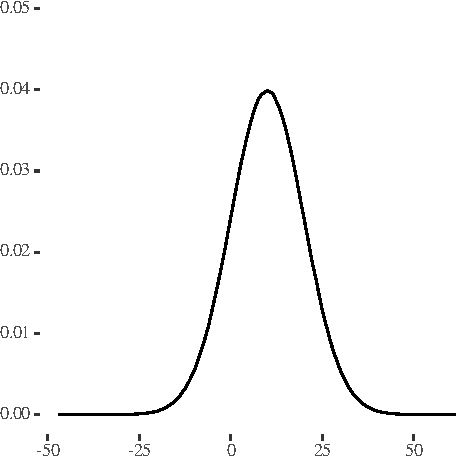
\includegraphics{bxjs_template_files/figure-latex/unnamed-chunk-2-1} 

}

\caption{アイリスデータセット}\label{fig:unnamed-chunk-2}
\end{figure}

\end{document}
